\chapter{Verification of models in LAMMPS}
In this chapter, i verify that my LAMMPS setup reproduces known results from the literature. This is necessary to trust the model to go further with modifications.

I use potentials that are already parts of the LAMMPS distribution, so I only need to test that I use LAMMPS correcty. 

\section{TIP4P/ICE}
I want to check that the TIP4P/ICE water potential in LAMMPS reproduces known thermodynamic properties from the literature. The TIP4P potential that comes with lammps, really just handles the massless charged site; the rest of the implementation, namely the rigid bonds and angle, are implemented by the user. Additionally, parameters have to be set. If thermodynamic properties are reproduces, I can be confident that my configuration of the TIP4P potential in LAMMPS is really the potential introduced by \cite{Abascal2005}. 
\subsection{Density of bulk water}
As a quick check of my TIP4P/ICE setup, I want to check the density of bulk water. This property is easily measured, as long as the simulation time is sufficient to gather enough statistics. 

\begin{table}
\centering
\caption{Liquid densities at melting points and melting points for several rigid water models at $P = \text{\SI{1}{\bar}}$. Adapted from \cite{Abascal2005}}
\begin{tabular}{c|cc}
Model & Melting point [K] & Density [\si{\gram\per\cubic\cm}] \\
\hline
TIP4P/ICE 	& 272.2 	& 0.985 \\
TIP4P 		& 232.0 	& 1.002 \\
TIP4P/Ew 	& 245.5 	& 0.992 \\
SPC/E 		& 215.0 	& 1.011 \\
Expt. 		& 273.15 	& 0.999
\end{tabular}
\end{table}

\section{United atom methane}
\section{Stabilizing methane hydrates}
The TIP4P/ICE potential should be able to stabilize a methane hydrate stucture. Therefore, I prepared an S1 hydrate using positions from \cite{Takeuchi2013}. These positions were derived using the TIP4P potential, so this configuration is not expected to be an equilibrium configuration for TIP4P/ICE. The hydrate equilibrated nicely, using a Nosé-Hoover $NPT$ thermostat with a temperature rising from $0$ to \SI{30}{\kelvin}. 

\begin{figure}
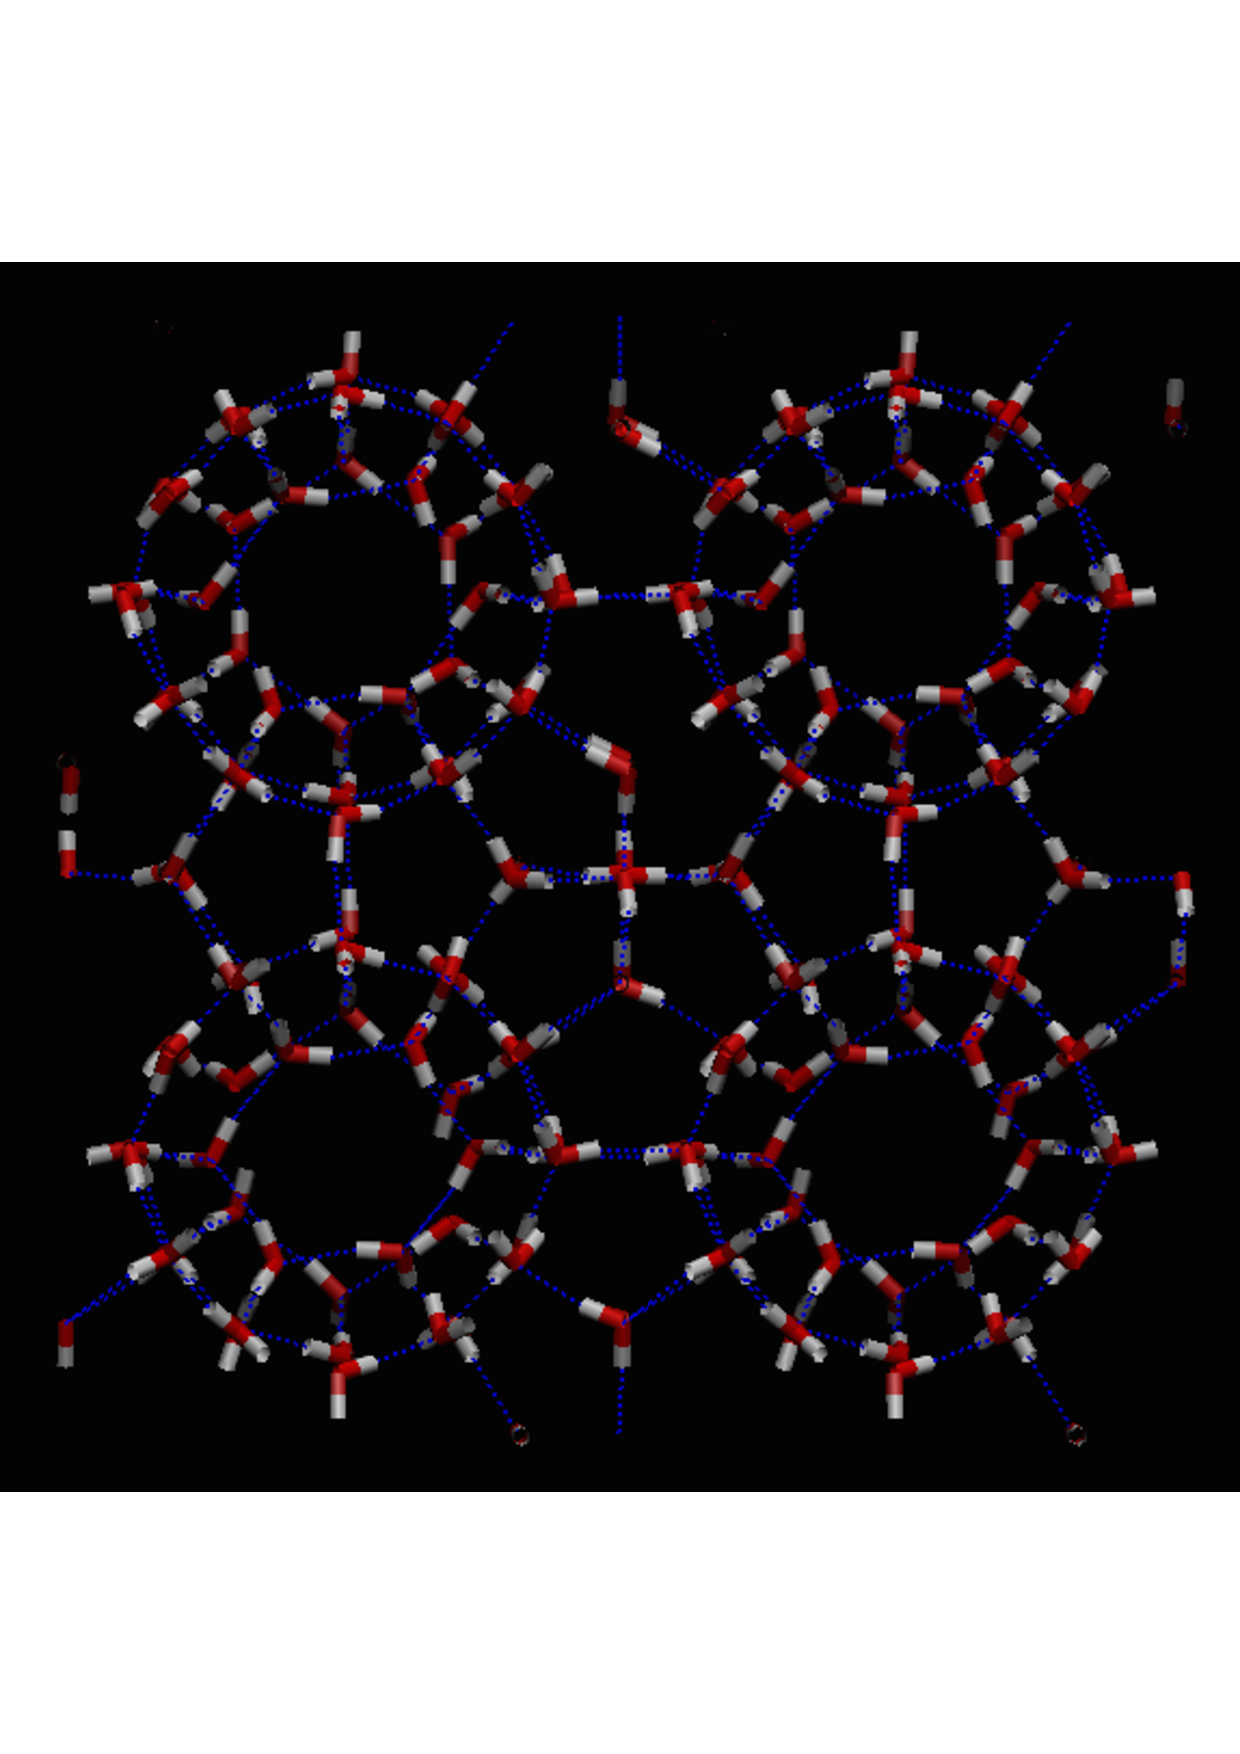
\includegraphics[width=\textwidth]{../snapshots/first_stable_hydrate.pdf}
\caption{Methane hydrate at low temperature. Rendered with VMD}
\label{fig:part2:first_hydrate}
\end{figure}

\section{Three-phase equilibrium line for methane hydrate}
Three-phase equilibrium simulations have been performed to check whether the model system is in the same ballpark as systems from the literature. Simulations have been performed on a system similar to the one in \cite{Conde2010}.

\section{Nucleation of methane hydrates?}
Nucleation of methane hydrates in a solution of water and methane is a rare event, and microsectond-simulations are required. 
